\documentclass[10pt]{scrartcl}
\usepackage[mdthm,colorsec,noauthor,noasy]{evan}
\usepackage{handout}
\usepackage[T1]{fontenc}
\usepackage{lmodern}
\usepackage{listings}
\lstset{language=Python,emptylines=1,basicstyle=\ttfamily\normalsize,identifierstyle=\color{black},keywordstyle=\color{NavyBlue},commentstyle=\color{black!60},stringstyle=\color{RawSienna},showstringspaces=false,columns=fullflexible,keepspaces=true,upquote=true,aboveskip=5pt,belowskip=5pt}
\newcommand{\py}[1]{\texttt{#1}}
\newcommand{\codeblock}[1]{\par\noindent\begin{minipage}{\linewidth}\csname code#1\endcsname\end{minipage}\par}
% Generated source-line references; regenerate after any Python edit.
\expandafter\def\csname coderace_source\endcsname{\lstinputlisting[firstline=4,lastline=12]{discussion_solutions.py}}
\expandafter\def\csname codefizzbuzz\endcsname{\lstinputlisting[firstline=16,lastline=27]{discussion_solutions.py}}
\expandafter\def\csname codeprime\endcsname{\lstinputlisting[firstline=31,lastline=39]{discussion_solutions.py}}
\expandafter\def\csname codeunique\endcsname{\lstinputlisting[firstline=43,lastline=58]{discussion_solutions.py}}
\expandafter\def\csname codebottles\endcsname{\lstinputlisting[firstline=62,lastline=70]{discussion_solutions.py}}
\expandafter\def\csname codedouble_trouble\endcsname{\lstinputlisting[firstline=74,lastline=81]{discussion_solutions.py}}
\expandafter\def\csname coderepeating\endcsname{\lstinputlisting[firstline=85,lastline=95]{discussion_solutions.py}}
\expandafter\def\csname codeclassify\endcsname{\lstinputlisting[firstline=4,lastline=15]{exam_solutions.py}}
\expandafter\def\csname codelong_groups\endcsname{\lstinputlisting[firstline=19,lastline=29]{exam_solutions.py}}
\expandafter\def\csname codegap\endcsname{\lstinputlisting[firstline=33,lastline=42]{exam_solutions.py}}
\expandafter\def\csname codelong_groups_stub\endcsname{\lstinputlisting[firstline=4,lastline=14]{exam_stubs.py}}
\expandafter\def\csname codegap_stub\endcsname{\lstinputlisting[firstline=18,lastline=27]{exam_stubs.py}}
\expandafter\def\csname codeprint_once\endcsname{\lstinputlisting[firstline=4,lastline=11]{examples.py}}
\expandafter\def\csname codebasic_reading\endcsname{\lstinputlisting[firstline=15,lastline=26]{examples.py}}
\expandafter\def\csname codefib\endcsname{\lstinputlisting[firstline=30,lastline=37]{examples.py}}
\expandafter\def\csname codeprime_factors\endcsname{\lstinputlisting[firstline=41,lastline=52]{examples.py}}
\expandafter\def\csname codepressure\endcsname{\lstinputlisting[firstline=56,lastline=59]{examples.py}}
\expandafter\def\csname codesums\endcsname{\lstinputlisting[firstline=63,lastline=84]{examples.py}}
\expandafter\def\csname codeapply_twice\endcsname{\lstinputlisting[firstline=88,lastline=89]{examples.py}}
\expandafter\def\csname codeadder\endcsname{\lstinputlisting[firstline=93,lastline=100]{examples.py}}
\expandafter\def\csname codecompose\endcsname{\lstinputlisting[firstline=104,lastline=107]{examples.py}}
\expandafter\def\csname codelambda\endcsname{\lstinputlisting[firstline=111,lastline=112]{examples.py}}
\expandafter\def\csname codecurry\endcsname{\lstinputlisting[firstline=116,lastline=139]{examples.py}}
\expandafter\def\csname codetrace\endcsname{\lstinputlisting[firstline=143,lastline=152]{examples.py}}
\expandafter\def\csname codeimprove\endcsname{\lstinputlisting[firstline=156,lastline=171]{examples.py}}
\expandafter\def\csname codesqrt\endcsname{\lstinputlisting[firstline=175,lastline=184]{examples.py}}
\expandafter\def\csname codenewton\endcsname{\lstinputlisting[firstline=188,lastline=197]{examples.py}}
\expandafter\def\csname coderoots\endcsname{\lstinputlisting[firstline=201,lastline=221]{examples.py}}
\expandafter\def\csname codetwenty_one\endcsname{\lstinputlisting[firstline=225,lastline=246]{examples.py}}
\expandafter\def\csname codeprinted\endcsname{\lstinputlisting[firstline=250,lastline=255]{examples.py}}
\expandafter\def\csname codehog_setup\endcsname{\lstinputlisting[firstline=3,lastline=4]{hog_solutions.py}}
\expandafter\def\csname coderoll_dice\endcsname{\lstinputlisting[firstline=8,lastline=20]{hog_solutions.py}}
\expandafter\def\csname codeboar\endcsname{\lstinputlisting[firstline=24,lastline=27]{hog_solutions.py}}
\expandafter\def\csname codetake_turn\endcsname{\lstinputlisting[firstline=31,lastline=37]{hog_solutions.py}}
\expandafter\def\csname codehog_helpers\endcsname{\lstinputlisting[firstline=41,lastline=65]{hog_solutions.py}}
\expandafter\def\csname codesus\endcsname{\lstinputlisting[firstline=69,lastline=89]{hog_solutions.py}}
\expandafter\def\csname codehog_play\endcsname{\lstinputlisting[firstline=93,lastline=104]{hog_solutions.py}}
\expandafter\def\csname codealways\endcsname{\lstinputlisting[firstline=108,lastline=112]{hog_solutions.py}}
\expandafter\def\csname codeis_always\endcsname{\lstinputlisting[firstline=116,lastline=126]{hog_solutions.py}}
\expandafter\def\csname codeaveraged\endcsname{\lstinputlisting[firstline=130,lastline=137]{hog_solutions.py}}
\expandafter\def\csname codemax_rolls\endcsname{\lstinputlisting[firstline=141,lastline=149]{hog_solutions.py}}
\expandafter\def\csname codeboar_strategy\endcsname{\lstinputlisting[firstline=153,lastline=156]{hog_solutions.py}}
\expandafter\def\csname codesus_strategy\endcsname{\lstinputlisting[firstline=160,lastline=164]{hog_solutions.py}}
\expandafter\def\csname codefinal_strategy\endcsname{\lstinputlisting[firstline=168,lastline=172]{hog_solutions.py}}
\expandafter\def\csname codehw_helpers\endcsname{\lstinputlisting[firstline=3,lastline=15]{hw_solutions.py}}
\expandafter\def\csname codeproduct\endcsname{\lstinputlisting[firstline=19,lastline=24]{hw_solutions.py}}
\expandafter\def\csname codeaccumulate\endcsname{\lstinputlisting[firstline=28,lastline=43]{hw_solutions.py}}
\expandafter\def\csname coderepeater\endcsname{\lstinputlisting[firstline=47,lastline=53]{hw_solutions.py}}
\expandafter\def\csname codecomposite\endcsname{\lstinputlisting[firstline=57,lastline=60]{hw_solutions.py}}
\expandafter\def\csname codechurch_basic\endcsname{\lstinputlisting[firstline=64,lastline=84]{hw_solutions.py}}
\expandafter\def\csname codechurch_arithmetic\endcsname{\lstinputlisting[firstline=88,lastline=97]{hw_solutions.py}}
\expandafter\def\csname codelab_print\endcsname{\lstinputlisting[firstline=4,lastline=12]{lab_solutions.py}}
\expandafter\def\csname codelab_if\endcsname{\lstinputlisting[firstline=16,lastline=32]{lab_solutions.py}}
\expandafter\def\csname codepick_digit\endcsname{\lstinputlisting[firstline=36,lastline=38]{lab_solutions.py}}
\expandafter\def\csname codemiddle\endcsname{\lstinputlisting[firstline=42,lastline=44]{lab_solutions.py}}
\expandafter\def\csname codefalling\endcsname{\lstinputlisting[firstline=48,lastline=53]{lab_solutions.py}}
\expandafter\def\csname codedivisible\endcsname{\lstinputlisting[firstline=57,lastline=62]{lab_solutions.py}}
\expandafter\def\csname codedouble_eights\endcsname{\lstinputlisting[firstline=66,lastline=71]{lab_solutions.py}}
\expandafter\def\csname codesum_digits\endcsname{\lstinputlisting[firstline=75,lastline=79]{lab_solutions.py}}

\title{CS 61A --- Week 2}
\subtitle{August 31--September 6: Control, Higher-Order Functions, Environments\\Composing Programs 1.4--1.6; Lab1, Discussion1, HW2, Hog}
\author{}\date{}\ihead{}
\begin{document}\maketitle
\section{Choose which statements run}
\begin{qbox}
Why does a second \py{if} sometimes run after the first, while an \py{elif} does not? Why can \py{0 and 1/0} finish without an error?
\end{qbox}
\textbf{Week 1 tools.} A call evaluates its operator, then arguments left to right, then applies the function. Assignment evaluates all right-hand values before changing bindings. A user-defined function call gets a new local frame. \py{print} has an output effect and returns \py{None}; \py{return} ends the current call. An expression statement such as \py{mul(x,x)} discards its computed value. The lab's \py{what\_prints} prints \py{Hello World!}, returns \py{'Goodbye.'}, then has an unreachable later print. At the prompt, the returned string appears with quotes; printing a string displays its text without quotes. These rules remain unchanged.

A \textbf{compound statement} consists of clauses, each with a colon-ended header and an indented suite of statements. Suites execute in order; a return redirects control immediately. Use consistent spaces for indentation. In \py{if}/\py{elif}/\py{else}, execute only the first true clause, or \py{else} if none is true. Two separate \py{if} statements make two separate choices.
\begin{example*}[Lecture 3, slide7]
For $ x=10$, separate tests \py{if x > 2} and \py{if x > 0} print both \py{big} and \py{positive}. An \py{if x > 2}/\py{elif x > 0} chain prints only \py{big}. For $ x=1$ the chain prints \py{less big}; for $ x=-1$ its \py{else} prints \py{not pos}. A negative number is true in a Boolean context even though \py{x > 0} is false.
\end{example*}
A \textbf{Boolean context} uses a value's truth to choose control. Among values seen so far, \py{False}, numeric zero, \py{''} (empty text), and \py{None} are false; other numbers and nonempty strings are true. Comparisons \py{< > <= >= == !=} produce \py{True}/\py{False}; \py{=} assigns instead of comparing.
\begin{proposition*}[Short-circuit rules --- Lectures3--4; CP1.5]
\begin{tabular}{p{.26\linewidth}p{.64\linewidth}}
\py{a and b}&Evaluate \py{a}; if false, return that value and skip \py{b}; otherwise evaluate and return \py{b}.\\
\py{a or b}&Evaluate \py{a}; if true, return that value and skip \py{b}; otherwise evaluate and return \py{b}.\\
\py{not a}&Evaluate \py{a}; return the Boolean opposite of its truth value.
\end{tabular}
\end{proposition*}
\par\noindent\begin{minipage}{\linewidth}
\begin{steps}
\ii In \py{0 and 1/0}, the first operand is false, so the result is $0$; division is never attempted. In \py{2 or 1/0}, the result is $2$ for the same reason with a true first operand.
\ii \py{2 and 7} returns $7$, \py{0 or 7} returns $7$, and \py{not 0} returns \py{True}. Only \py{not} must return a Boolean rather than an operand value.
\ii These operators are not ordinary two-argument function calls: an ordinary call evaluates \emph{both} argument expressions before applying its function.
\end{steps}
\end{minipage}\par
\method{Printing a function result exactly once --- Lecture3, slides4--5.}
For a pure \py{f(x)} returning $ x+1$, compare the following bodies when called on $3$:
\begin{center}\begin{tabular}{l|l|l}
Body&printed lines&return value\\\hline
\py{return f(x)}&none&$4$\\
\py{print(f(x))}&\py{4}&\py{None}\\
\py{f(x)}&none&\py{None}\\
\py{return print(f(x))}&\py{4}&\py{None}
\end{tabular}\end{center}
To print \emph{and} return the result, store it once. Here \py{f} is supplied as an argument; \py{increment} is the pure example.
\codeblock{print_once}
\py{print\_once(2, increment)} prints $3$ and returns $3$. Writing \py{print(f(x))} followed by \py{return f(x)} instead calls \py{f} twice. If \py{f = print}, that repeats its output effect. Lecture3 slide5's caption labels the twice-called version C; the actual twice-called code is B.
\begin{shortcuts}
\ii To check a long \py{and}/\py{or} expression, mark which operand is reached next and whether its truth value is already decisive. Do not evaluate a skipped error-producing call.
\ii Separate the printed lines from the returned value, as in Week1. A bare expression inside a function is not automatically returned.
\end{shortcuts}
\begin{trapbox}
\ii \py{5 and 2} is $2$, not \py{True}. ``And means both true'' describes its truth, not its returned value.
\ii An \py{elif c > 7} after \py{if c > 5} can never run: every input satisfying the later test already satisfies the first.
\end{trapbox}

\section{Describe what each loop variable means}
\begin{qbox}
How do we know that a Fibonacci loop returns the requested term, rather than the term before it? How does $858$ become the factors $2,3,11,13$?
\end{qbox}
\begin{proposition*}[Iteration and its maintained property --- CP1.5; Lecture3]
A \py{while} statement tests its condition before every iteration. A true condition runs the entire body, then the test repeats; a false condition continues after the loop. A \textbf{loop invariant} is a property true before every test. Prove it initially, show one iteration preserves it, then use the stopping condition to identify the result. Termination needs a separate reason.
\end{proposition*}
\Needspace{11\baselineskip}
Define $ F_0=0$, $ F_1=1$, and $ F_{k+1}=F_k+F_{k-1}$ for $ k\ge1$.
\begin{motive}
\ii[Want.] Choose enough variables to remember the progress already made.
\ii[Know.] The next Fibonacci term depends on the previous two terms, not the entire earlier sequence.
\ii[Key step.] Store two consecutive values and their index: before each test, \py{pred} is $ F_{k-1}$ and \py{curr} is $ F_k $. Update both from their old values, then increase the index.
\end{motive}
\codeblock{fib}
\begin{fig}
\begin{tikzpicture}[every node/.style={font=\normalsize},box/.style={draw=NavyBlue,fill=NavyBlue!4,align=center,inner sep=5pt}]
\node[box] (a) at (0,0) {$ k=1$\\$(\mathrm{pred},\mathrm{curr})=(0,1)$};
\node[box] (b) at (4,0) {$ k=2$\\$(1,1)$};
\node[box] (c) at (7.4,0) {$ k=3$\\$(1,2)$};
\node[box] (d) at (10.1,0) {$ k=4$\\$(2,3)$};
\draw[-{Latex}] (a)--(b);\draw[-{Latex}] (b)--(c);\draw[-{Latex}] (c)--(d);
\end{tikzpicture}
\figcap{The pair changes from $(F_{k-1},F_k)$ to $(F_k,F_{k-1}+F_k)$. Both right-hand values must use the old pair.}
\end{fig}
\par\noindent\begin{minipage}{\linewidth}
\begin{steps}
\ii Initially $ k=1$, so $(0,1)=(F_0,F_1)$. One update preserves the property by the defining recurrence.
\ii Each iteration increases $ k $ by $1$. For integer $ n\ge1$, it reaches $ k=n $, where the condition is false and \py{curr} is $ F_n $.
\ii Thus \py{fib(1)}$=1$, \py{fib(3)}$=2$, \py{fib(8)}$=21$, \py{fib(50)}$=12586269025$. At $ n=1$, the body never runs.
\end{steps}
\end{minipage}\par
\begin{example*}[Lecture3 slide9: finish the whole body]
Starting with \py{i, total = 0, 0}, the loop \py{while i < 3} executes \py{i = i + 1} and then \py{total = total + i}. The pairs after complete iterations are $(1,1),(2,3),(3,6)$. Updating \py{i} to $3$ does not skip the remaining addition in that iteration; only the \emph{next} test stops it.
\end{example*}
\method{Prime factorization --- Lecture3.}
An integer at least $2$ is \textbf{prime} if its only positive divisors are $1$ and itself; it is \textbf{composite} if it has a divisor strictly between them. The smallest divisor above $1$ of an integer $ n>1$ is prime: a composite divisor would have a smaller divisor at least $2$. Find that divisor, print it, and divide it out. (Week1 used the same search to find the largest proper partner.)
\codeblock{prime_factors}
\begin{center}\begin{tabular}{c|c|c|c}
remaining \py{n}&smallest divisor \py{k}&printed so far&new remaining \py{n}\\\hline
858&2&$2$&429\\429&3&$2,3$&143\\143&11&$2,3,11$&13\\13&13&$2,3,11,13$&1
\end{tabular}\end{center}
\Needspace{7\baselineskip}
Each step preserves ``original input = product of printed factors $\times $ remaining \py{n}''. The remaining positive integer strictly decreases, so it reaches $1$. Factors appear in nondecreasing order: a smaller divisor of the new remainder would already have divided the old one. Source examples: $8=2^3$, $9=3^2$, $10=2\cdot5$, $11$ is prime, $12=2^2\cdot3$. For input $1$, print nothing.

\method{Read decimal digits with quotient and remainder --- Lab1; Discussion1.}
For integer $ n\ge0$ and $ d>0$, uniquely $ n=dq+r $ with $0\le r<d $. Python gives $ q=n//d $, $ r=n\%d $. Thus \py{n \% 10} is the last digit, \py{n // 10} removes it, and \py{(n // 10**k) \% 10} extracts position $ k $ from the right. For $3579$, division by $100$ gives $35$, and remainder by $10$ gives digit $5$.
\begin{center}\begin{tabular}{c|ccc}
 &\py{/}&\py{//}&\py{\%}\\\hline
$1,5$&$0.2$&$0$&$1$\\$25,4$&$6.25$&$6$&$1$\\$4,2$&$2.0$&$2$&$0$
\end{tabular}\end{center}
All three operations raise \py{ZeroDivisionError} for divisor zero. Floor division with negative inputs still rounds downward: \py{-5 // 4} $= -2$, not $-1$; the decimal-digit methods here use nonnegative integers.
\begin{example*}[A stopping test must detect passing, not just equality --- Discussion1 Q1]
The source race loop continues while \py{(minutes == 0) or (tortoise - hare)}. Every nonzero difference is true, including one showing the tortoise has already passed the hare. For speeds $(2,3)$, the hare travels $15$ feet in its first five minutes and rests; at minute8 the tortoise is at $16$, but the code continues and returns $15$ minutes, when both distances equal $30$. Test whether the tortoise is \emph{still behind} instead. The worksheet's equality examples use ``catches up'' as $\ge $, despite its conflicting phrase ``greater distance.''
\end{example*}
\begin{shortcuts}
\ii For a digit loop, write the unprocessed number and the accumulated answer separately. Removing one last digit decreases a positive integer, proving termination.
\ii To recognize adjacent eights, inspect \py{n \% 100 == 88}, then remove just \emph{one} digit so that overlapping pairs are checked.
\ii A factor-count loop includes $ n $ itself; a proper-factor sum stops before $ n $. The different bounds reflect the different tasks, rather than a different loop rule.
\end{shortcuts}
\begin{trapbox}
\ii A changed variable need not move toward a false condition. Specify a bound or decreasing nonnegative quantity.
\ii In the block-repetition task, \py{repeating(t,n)} tests whether $ n $ is a repetition of a $ t $-digit positive integer. Blocks need their stated width. A last-two-digit block $01$ has numeric remainder $1$; the source's natural blank fills wrongly accept \py{repeating(2,101)}. Require the final block to have two digits before comparing blocks.
\end{trapbox}

\section{State a function's job and test its contract}
\begin{qbox}
What does omitting an argument mean? How can a test detect an off-by-one loop without testing every input?
\end{qbox}
\textbf{Design --- CP1.4; Lecture4.} Give a function one job, reuse a shared computation instead of copying it, and make the function apply to related inputs. A contract states its domain, return values, and effects. For real inputs, \py{square} returns a nonnegative real square; this does not assert the same ordered property for complex numbers. \textbf{Modularity} divides a program into parts with specific jobs; \textbf{abstraction} lets a caller use a contract; \textbf{separation of concerns} lets one part change without rewriting another's job.
\codeblock{pressure}
This is the reading's ideal-gas formula $ P=nkT/V $ (cited physical model), with volume in cubic metres, temperature in kelvin, and particle count $ n $. The \textbf{default argument} \py{n=6.022e23} is recorded when the function is defined and used if the call omits that argument. Supplying it overrides the default. A \textbf{keyword argument} names the parameter in the call, as in \py{pressure(v=1,t=273.15)}; positional arguments must come before named ones. The assignment \py{k = 1.38e-23} instead runs inside each call. A \textbf{docstring} documents the function and is shown by \py{help(pressure)}; a \py{\#} comment is for readers of the source and is ignored during execution.
\begin{example*}[CP1.4 and Lecture4 slide6]
\py{pressure(1,273.15)} returns $2269.974834$; supplying \py{3 * 6.022e23} as the third argument returns $6809.924502$. For the built-in rounding function: \py{round(1.23,1)} is $1.2$; \py{round(1.23,0)} is \py{1.0}; \py{round(1.23,5)} is $1.23$; \py{round(1.23)} is integer $1$. The slide drops the decimal in the second example; Python preserves a floating-point result there.
\end{example*}
\method{Assertions and doctests --- CP1.5.}
\py{assert fib(8) == 21, 'wrong Fibonacci value'} does nothing if the comparison is true; otherwise it raises \py{AssertionError} with the message. A \textbf{unit test} checks one function. Test ordinary inputs and boundaries: $ n=1,3,50$ check the Fibonacci loop's zero-iteration case, early progress, and a larger result. A docstring's \py{>>>} examples specify both displayed output and return values; \py{python3 -m doctest file.py} checks them. Programmatically, \py{doctest.testmod()} checks a module's examples; \py{doctest.run\_docstring\_examples(f, globals(), True)} checks one function with verbose output. Here \py{globals()} supplies current global bindings to the examples. The reading tests its loop-based \py{sum\_naturals}, which sums $1$ through $ n $, at $10$ and $100$, expecting $55$ and $5050$. Passing tests checks those examples; the loop-property argument proves the algorithm for its stated domain.

The reading's \py{percent\_difference(40,50)} computes $100|40-50|/40=25.0$ (first input must be nonzero). Its absolute-value example uses the negative, zero and positive branches explicitly:
\codeblock{basic_reading}
Lecture4's \py{get\_name(first,last)} returns \py{first} if it is nonempty, otherwise \py{last}; \py{get\_name('', 'Ousterhout')} gives \py{'Ousterhout'}. Its \py{same\_length(a,b)} repeatedly divides each positive integer by $10$ and compares digit counts: $(4,8)$ and $(100,657)$ give true; $(4,100)$ gives false. That source implementation counts zero as zero digits, so use its positive-integer domain rather than claiming it handles every integer.
\begin{shortcuts}
\ii Distinguish optional arguments from required ones by the signature. For \py{pressure}, omitting the particle count uses the recorded default; a supplied count overrides it.
\ii Test a loop that should run zero times, one time, and several times; these cases expose initialization and stopping mistakes.
\end{shortcuts}
\begin{trapbox}
\ii A default is not reassigned on every call. A local assignment and a default parameter use \py{=} in different execution rules.
\ii A printed number is not a returned number. Tests that bind \py{a = divisible\_by\_k(...)} check the count returned separately from the printed multiples.
\end{trapbox}

\section{Pass the changing operation as a function}
\begin{qbox}
The loops for $1+\cdots+n $, $1^3+\cdots+n^3$ and a pi approximation differ in just one term. Can one loop express all three?
\end{qbox}
A \textbf{higher-order function} accepts a function as an argument or returns a function. Functions are \textbf{first-class values}: they can be named, passed, returned, and stored in collections (the last use is studied later). A parameter can therefore be bound to a function just as it can be bound to a number.
\begin{motive}
\ii[Want.] Avoid copying the same summation loop for each formula.
\ii[Know.] The initial total, index, stopping test and addition stay the same; only the value added at index $ k $ changes.
\ii[Key step.] Supply a one-argument function \py{term}; use \py{term(k)} where the differing expression used to be. Bind \py{term} to the function itself, not to one already-computed term.
\end{motive}
\codeblock{sums}
\begin{fig}
\begin{tikzpicture}[every node/.style={font=\normalsize},box/.style={draw=NavyBlue,fill=NavyBlue!4,align=left,inner sep=6pt}]
\node[box] (s) at (0,0) {\py{summation(3,cube)}\\\py{n}: $3$; \py{term}: function \py{cube}\\$(k,\mathrm{total}): (1,0)\to(2,1)\to(3,9)\to(4,36)$};
\node[box] (c) at (6.8,0) {\py{term(2)} calls \py{cube(2)}\\new local \py{x}: $2$\\returns $8$};
\draw[-{Latex}] (s)--(c);
\end{tikzpicture}
\figcap{At each index, the same binding \py{term}$\to $\py{cube} computes a new value. Before the next test, the total includes exactly the terms already visited.}
\end{fig}
\par\noindent\begin{minipage}{\linewidth}
\begin{steps}
\ii Before the test at index $ k $, \py{total} equals $\sum_{j=1}^{k-1}\mathrm{term}(j)$. Initially it is the empty sum $0$.
\ii Adding \py{term(k)} and increasing $ k $ preserves that property. At $ k=n+1$, it gives the complete sum. For $ n=0$, the result is $0$ without calling \py{term}.
\ii \py{summation(100,identity)} is $5050$; \py{summation(100,cube)} is $25502500$; \py{summation(10,square)} is $385$. Lecture4's five cubes sum to $225$; a separate \py{cube(7)} call returns $343$.
\end{steps}
\end{minipage}\par
\begin{example*}[The reading's pi sum]
Its $ k $ th term is $8/((4k-3)(4k-1))$. With $100$ terms the sum is $3.1365926848388144$; with $10^6$ terms it is $3.141592153589902$. The analytical claim that these sums converge to $\pi $ is cited from the reading; the code computes the stated finite sums. The original three standalone loops are exactly this common loop with the corresponding term expression substituted.
\end{example*}
\method{Change addition into a supplied combination --- HW2 Q1--Q2.}
\py{from operator import add, mul} supplies two-argument addition and multiplication functions. A product loop starts at $1$, because multiplying no factors should leave the multiplicative identity. For a general two-argument \py{fuse}, start at \py{start} and repeatedly replace \py{result} with \py{fuse(result,term(k))}. This is \py{accumulate}. HW2 assumes associativity and commutativity; its nested combination can then be evaluated in this left-to-right order. For \py{accumulate(add,11,3,square)}, totals are $11\to12\to16\to25$. For multiplication with start $=2$, they are $2\to2\to8\to72$. With zero terms, return the unchanged start and never call either function.
Lecture5 defines the repeated-call helper as follows:
\codeblock{apply_twice}
\begin{shortcuts}
\ii Summation uses combination \py{add} and start $0$; product uses \py{mul} and start $1$. The identities explain the two one-line wrappers.
\ii \py{apply\_twice(square,2)} gives $\py{square}(\py{square}(2))=16$: the same function value is used twice, in separate call frames.
\end{shortcuts}
\begin{trapbox}
\ii \py{summation(5,cube(5))} passes $125$, then tries to call it. \py{summation(5,cube)} passes the required function.
\ii The name \py{term} is a local binding, not necessarily the function's original name. Looking up its value uses the same rule as any other parameter.
\end{trapbox}

\section{A returned function retains its defining environment}
\begin{qbox}
After \py{three\_more\_than = make\_adder(3)} returns, where does \py{three\_more\_than(4)} find the $3$?
\end{qbox}
\begin{proposition*}[Lexical scope --- Lecture5; CP1.6]
When a function is defined, record the current frame as its \textbf{parent}. Calling that function creates a local frame with this recorded parent. Name lookup follows those parent links, starting locally. The caller's frame is not substituted for the defining parent. A function retaining access to its enclosing bindings is a \textbf{closure}; returning it preserves that access.
\end{proposition*}
\codeblock{adder}
\begin{fig}
\begin{tikzpicture}[every node/.style={font=\normalsize},box/.style={draw=NavyBlue,fill=NavyBlue!4,align=left,inner sep=6pt}]
\node[box] (g) at (0,0) {\textbf{Global}\\\py{make\_adder} $\to $ function [parent=Global]\\\py{three\_more\_than} $\to $ \py{adder} [parent=f1]};
\node[box] (f1) at (0,-1.9) {\textbf{f1: \py{make\_adder(3)}}\\\py{n}: $3$; \py{adder} $\to $ function [parent=f1]};
\node[box] (f2) at (7,-1.9) {\textbf{f2: \py{adder(4)}}\\\py{k}: $4$\\return value $4+3=7$};
\draw[-{Latex},thick] (f2)--node[above]{parent} (f1);\draw[-{Latex},thick] (f1)--node[right]{parent} (g);
\end{tikzpicture}
\figcap{Lookup for \py{n} goes from f2 to f1 and finds $3$. The function's recorded parent keeps this binding available after \py{make\_adder} returns.}
\end{fig}
\par\noindent\begin{minipage}{\linewidth}
\begin{steps}
\ii Calling \py{make\_adder(3)} binds \py{n} in f1. Executing its nested \py{def} creates \py{adder} with parent f1; its body is not yet executed.
\ii Returning \py{adder} returns a function value. Calling that value on $4$ creates f2 with parent f1, so lookup finds local \py{k=4}, then enclosing \py{n=3}.
\ii A separate \py{make\_adder(5)} creates another enclosing frame and another function. It does not change the first closure's parent or its $3$.
\end{steps}
\end{minipage}\par
\begin{center}\begin{tabular}{p{.55\linewidth}|p{.37\linewidth}}
\textbf{Lecture5's changed line}&\textbf{Result of \py{add\_three(4)}}\\\hline
A: \py{k=5} in the enclosing \py{make\_adder}&$7$: the inner parameter \py{k=4} is found first.\\
B: \py{n=5} before defining \py{adder}&$9$: captured \py{n} is now $5$.\\
C: \py{k=5} inside \py{adder}&$8$: its local argument binding is replaced.\\
D: also create \py{add\_five=make\_adder(5)}&$7$: a separate defining frame.\\
E: \py{n=5} after nested \py{def}, before return&$9$: the closure uses the binding when called.\\
F: global \py{n=5} after \py{make\_adder(3)}&$7$: lookup finds the enclosing $3$ first.
\end{tabular}\end{center}
Moving \py{adder} out to global scope changes its parent to Global. If there is no global \py{n}, calling it raises \py{NameError}; the caller's local \py{n=3} cannot supply the missing binding. A closure retains access to bindings, not a rule that copies all free-variable values at definition time (variant E distinguishes these).

\method{Compose and repeat --- CP1.6; HW2 Q3--Q4.}
Composition applies \py{g} first, then \py{f}. The returned function's parent holds both function bindings.
\codeblock{compose}
The reading calls the increment function \py{successor}. \py{compose1(square,increment)(12)} gives $(12+1)^2=169$, even if an unrelated global function is named \py{f}. To repeat \py{f} $ n $ times, return a function with its own counter and current value: start at input $ x $, replace it by \py{f(x)} exactly $ n $ times, then return it. For three squares starting at $5$, the values are $5\to25\to625\to390625$. To test whether \py{f} and \py{g} agree in both composition orders at a particular $ x $, return a function computing \py{f(g(x)) == g(f(x))}; do not claim agreement for \emph{all} inputs from one test.

\method{Lambda creates a function value --- CP1.6.}
A \py{lambda parameters: expression} has one return expression and no assignment or control statements in its body. Creation does not evaluate that body; a later call does. Its recorded name is \py{<lambda>}; assigning another name does not rename it.
The following assignments rename the reading\textquotesingle s \py{s} and lambda-based \py{compose1}, keeping both implementations available.
\codeblock{lambda}
\py{square\_lambda(12)} is $144$; \py{compose\_lambda(lambda x:x*x, lambda y:y+1)(12)} is $169$. The shorter \py{compose\_lambda} has the same parent-link reasoning as the nested \py{def}; explicit definitions are often easier to read.

\method{Currying: choose arguments one call at a time --- CP1.6.}
\textbf{Currying} transforms a two-argument function into a function returning a one-argument function: \py{curry2(f)(x)(y)} computes \py{f(x,y)}. \textbf{Uncurrying} reverses that interface.
\codeblock{curry}
\py{curried\_pow(2)(3)} is $8$. Set \py{pow\_curried=curry2(pow)}: \py{pow\_curried(2)(5)} and \py{uncurry2(pow\_curried)(2,5)} are both $32$. \py{map\_to\_range(0,10,curried\_pow(2))} prints $1,2,4,8,16,32,64,128,256,512$, one per line. The outer call captures $2$; each inner call supplies a different exponent. The endpoint $10$ is excluded.

\method{A decorator replaces the function binding --- CP1.6.}
\codeblock{trace}
\Needspace{8\baselineskip}
The annotation \py{@trace} means: create the original \py{triple}, pass it to \py{trace}, then bind \py{triple} to the returned \py{wrapped} function. Thus \py{triple(12)} prints a trace line containing the original function and argument $12$, and returns $36$. The function's displayed memory address varies. This is equivalent to an undecorated definition followed by \py{triple = trace(triple)}. A decorator may itself be a call expression: evaluate that expression first, create the new function, then apply the resulting decorator to it.
\begin{shortcuts}
\ii For every nested definition, label its parent immediately. Copy that parent to each later call frame; this settles lookup even when the function is called elsewhere.
\ii Distinguish \py{return adder} (return the function) from \py{return adder(4)} (call it and return a number).
\ii For curried calls, evaluate each call from left to right: \py{curry2(pow)} returns a function, its \py{(2)} returns another, and \py{(5)} returns $32$.
\end{shortcuts}
\begin{trapbox}
\ii A global name with the same spelling cannot override an earlier matching binding in the parent chain. Conversely, a caller's unrelated local name is not searched.
\ii \py{composite\_identity(square,increment)(0)} is true ($1=1$), but at $4$ it is false ($25\ne17$). Its result concerns the supplied input.
\end{trapbox}

\section{Separate an iteration from its update rule}
\begin{qbox}
How can one loop approximate both the golden ratio and square roots, when the equations differ?
\end{qbox}
Supply two functions: an \py{update} that produces the next guess and a \py{close} test that decides when the current guess is acceptable. The reading compares numbers by an \emph{absolute tolerance}; $|x-y|<\varepsilon $ is its definition of approximate equality.
\codeblock{improve}
\begin{example*}[Golden ratio --- CP1.6]
The positive number $\phi $ satisfies $\phi=1+1/\phi $, equivalently $\phi^2=\phi+1$. Solving $ x^2-x-1=0$ gives $\phi=(1+\sqrt5)/2$. The update $ x\mapsto1+1/x $ gives
\[
1\to2\to1.5\to1.666666\ldots\to1.6\to1.625\to\cdots.
\]
The residual test compares $ x^2$ with $ x+1$. The printed source implementation returns $1.6180339887498951$; comparing this with the closed form at tolerance $10^{-15}$ passes.
\end{example*}
\method{Why this update approaches the positive solution in exact arithmetic.}
\par\noindent\begin{minipage}{\linewidth}
\begin{steps}
\ii Any positive initial guess maps first to a number greater than $1$, then into $(1,2)$. Subsequent guesses enter and stay in $[1.5,2]$.
\ii For $ x,\phi\in[1.5,2]$, the update error is
$|(1+1/x)-(1+1/\phi)|=|x-\phi|/(x\phi)\le(4/9)|x-\phi|$.
\ii Repeating shrinks the error by a geometric factor. This proves convergence in exact arithmetic; finite-precision stopping still depends on the tolerance and operations.
\end{steps}
\end{minipage}\par
\method{Capture the equation's parameter --- CP1.6 square root.}
An update \py{sqrt\_update(x,a)} has two inputs, but \py{improve} requires a one-input update. Put it inside \py{sqrt(a)} so that it can find \py{a} through its parent frame.
\codeblock{sqrt}
\par\noindent\begin{minipage}{\linewidth}
\begin{steps}
\ii For $ a>0$, a positive guess $ x $ and its quotient $ a/x $ lie on opposite sides of $\sqrt a $ unless already equal. Their average supplies a new positive guess. If $ r=\sqrt a $, then $(x+a/x)/2-r=(x-r)^2/(2x)\ge0$.
\ii After the first update, $ x\ge r $; the next average is at most $ x $ and at least $ r $, the next error is $(x-r)^2/(2x)\le(x-r)/2$. Repeating halves an upper bound on the error, so the exact guesses converge to $ r $.
\ii For \py{sqrt(256)}, the local update call looks up \py{x} in its own frame and \py{a=256} in the enclosing \py{sqrt} frame; it does not look up \py{a} in \py{improve}'s frame. The source example returns \py{16.0}.
\end{steps}
\end{minipage}\par

The \textbf{derivative} $ df(x)$ is the slope of the tangent line approximating the curve near $ x $.
\Needspace{15\baselineskip}
\begin{proposition*}[Newton update --- CP1.6]
Given a differentiable function $ f $ and its derivative $ df $, the tangent line at $ x $ is $ y=f(x)+df(x)(t-x)$. If $ df(x)\ne0$, its zero occurs at
\[
\boxed{x_{\mathrm{new}}=x-\frac{f(x)}{df(x)}.}
\]
This is an update rule, not a guarantee of convergence for arbitrary functions or initial guesses.
\end{proposition*}
\begin{motive}
\ii[Want.] Move a guess toward a zero of a curved function.
\ii[Know.] Near the guess, the tangent is a linear approximation. Solving the exact curved equation may be difficult; solving a linear equation is direct.
\ii[Key step.] Set the tangent's output to zero and solve for its input: $0=f(x)+df(x)(t-x)$. This suggests a new guess; check the original function again there.
\end{motive}
\begin{fig}
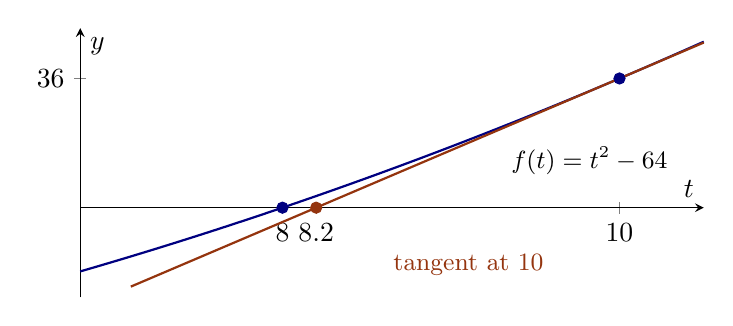
\begin{tikzpicture}
\begin{axis}[width=9.5cm,height=5cm,xmin=6.8,xmax=10.5,ymin=-25,ymax=50,axis lines=middle,xlabel={$ t $},ylabel={$ y $},xtick={8,8.2,10},xticklabels={$8$,$8.2$,$10$},ytick={36},samples=100,clip=false]
\addplot[NavyBlue,thick,domain=6.8:10.5]{x*x-64};
\addplot[RawSienna,thick,domain=7.1:10.5]{20*x-164};
\addplot[only marks,mark=*,NavyBlue] coordinates {(8,0)(10,36)};
\addplot[only marks,mark=*,RawSienna] coordinates {(8.2,0)};
\node[anchor=west,font=\small] at (axis cs:9.3,13){$ f(t)=t^2-64$};
\node[anchor=west,font=\small,text=RawSienna] at (axis cs:8.6,-16){tangent at $10$};
\end{axis}
\end{tikzpicture}
\figcap{At $ x=10$, $ f(x)=36$ and $ df(x)=20$. The tangent meets zero at $10-36/20=8.2$, closer to the curve's actual zero $8$.}
\end{fig}
\codeblock{newton}
\method{Roots of different degrees --- CP1.6.}
For positive integer $ n $ and $ a>0$, the equation $ x^n=a $ becomes the zero equation $ f(x)=x^n-a=0$. The calculus rule $ df(x)=nx^{n-1}$ is cited. For nonnegative integer $ n $, the power loop multiplies by $ x $ exactly $ n $ times; it returns $1$ for $ n=0$.
\codeblock{roots}
At $ a=64$, degrees $2,3,6$ give $8.0,4.0,2.0$: $8^2=4^3=2^6=64$. \py{square\_root\_newton(64)} also returns $8.0$.
\begin{shortcuts}
\ii To derive a Newton update, first write the desired equation as $ f(x)=0$, then solve the tangent equation. For $ x^2-a $, this gives $ x-(x^2-a)/(2x)=(x+a/x)/2$, the same average update.
\ii Nested helpers let a general one-input method use a fixed parameter: its value is stored in the enclosing frame, not added as another update argument.
\end{shortcuts}
\begin{trapbox}
\ii Near a zero, residual $|f(x)|$ and input error $|x-r|$ at a zero $ r $ are different quantities. For example, $ f(x)=10^{-6}x $ at $ x=1$ has residual $10^{-6}$ but input error $1$. A residual tolerance alone is not a universal bound on input error.
\ii Smaller tolerance need not make floating-point iteration finish. For $ a=10$, the average update can become unchanged at $3.162277660168379$, whose squared residual is about $-1.77636\cdot10^{-15}$: the source's $10^{-15}$ test keeps failing. Its iframe diagrams instead use $10^{-3}$; do not confuse those two tolerances.
\ii Newton can divide by zero, diverge, or alternate forever: for $ f(x)=x^3-2x+2$, initial guess $0$ updates to $1$, then back to $0$. A test on the successful $64$ examples does not prove general convergence.
\end{trapbox}

\section{Use function contracts to separate a game from its decisions}
\begin{qbox}
Can a simulator play the same game with different players, scoring rules and dice, without rewriting its turn loop?
\end{qbox}
\textbf{Lecture4's Twenty-One.} Start at total $=0$; alternate adding $1$, $2$, or $3$. The first player to make the total at least $21$ \emph{loses}. A strategy takes the current total and returns an allowed addition. The source's \py{simple\_strategy} adds $3$ below $15$, then $2$; its nested wrapper prints a supplied remark before calling the original strategy. The simulator below is the lecture's \py{play}, renamed to distinguish it from Hog.
\codeblock{twenty_one}
With two simple strategies, totals are $0,3,6,9,12,15,17,19,21$. Player1 makes the last addition and loses; the code has already switched \py{current\_player} to Player0, so it prints \py{Player 0 wins the game}. The lecture's \py{interactive\_strategy} prints the current score, reads text with \py{input()}, and converts it using \py{int}; only the strategy changes, not the simulator.

\subsection{Hog: define a die, a turn, and a score update}
\begin{qbox}
If a die rolls a $1$ on the second of five required rolls, can the simulator stop rolling immediately?
\end{qbox}
\textbf{P0: die interface.} A die is a supplied zero-argument function returning a positive integer outcome. A fair six-sided die returns $1$--$6$ with equal probabilities. The supplied \py{make\_test\_dice(4,1,2)} returns a stateful test die whose successive calls return $4,1,2,4,1,\ldots $. Its implementation uses later features; its documented interface is enough here. Each call advances its state, so repeated calls are observable effects.

\textbf{Rules.} Two players alternate turns toward a goal (default $100$). A strategy takes the current player's score and the opponent's score and returns a roll count $0$--$10$. For positive rolls, \textbf{Sow Sad} awards $1$ if any roll is $1$; otherwise award the sum. For zero rolls, \textbf{Boar Brawl} awards
\[
\max\bigl(1,3|\text{opponent's tens digit}-\text{own ones digit}|\bigr).
\]
Then \textbf{Sus Fuss} applies to the \emph{new total}: if it has exactly $3$ or $4$ positive factors, replace it with the next greater prime. A \textbf{prime} is an integer at least $2$ with exactly the positive divisors $1$ and itself. Both $1$ and the number count as factors. The game ends at the end of a turn when a total reaches or exceeds the goal.
\begin{example*}[Actual Hog examples]
Seven dice with five $1$ s score $1$; four $3$ s score $12$. Zero-roll scores for own/opponent totals $(21,46)$, $(45,52)$ and $(2,5)$ are $9,1,6$. A total $14+7=21$ has factors $1,3,7,21$, so it becomes $23$; $63+1=64$ has seven factors and stays $64$; $49+18=67$ is prime and stays $67$.
\end{example*}
\begin{fig}
\begin{tikzpicture}[every node/.style={font=\normalsize},box/.style={draw=NavyBlue,fill=NavyBlue!4,align=center,inner sep=6pt}]
\node[box] (a) at (0,0) {own $14$, opponent $20$\\strategy returns $2$ rolls};
\node[box] (b) at (5,0) {die calls: $3$, then $4$\\turn points $=7$};
\node[box] (c) at (9.2,0) {new total $21$\\Sus Fuss $\to23$};
\draw[-{Latex}] (a)--(b);\draw[-{Latex}] (b)--(c);
\end{tikzpicture}
\figcap{A strategy chooses a roll count; a turn produces points; an update returns a new total. Confusing these three return values causes different errors.}
\end{fig}
\method{Derive each simulator function from its contract --- P1--P5.}
\par\noindent\begin{minipage}{\linewidth}
\begin{steps}
\ii \py{roll\_dice} records a sum and whether any $1$ occurred. Make \emph{every} requested die call, then return $1$ or the sum. Early return on the first $1$ would leave a test die at the wrong point in its cycle.
\ii \py{boar\_brawl} extracts \py{score \% 10} and \py{(opponent // 10) \% 10}; the latter must retain only the tens digit even above $99$. \py{take\_turn} dispatches zero rolls here and positive rolls to \py{roll\_dice}.
\ii \py{num\_factors} counts divisors $1$ through $ n $. \py{sus\_points} advances from a sus total until the supplied positive-integer \py{is\_prime} test passes. \py{sus\_update} adds turn points to the old total \emph{before} applying Sus Fuss. The next-prime search terminates because primes exist above every integer (cited number-theory fact).
\ii \py{play} stores both scores and whose turn is next. On each turn, call only that player's strategy once, pass its result to the update once, replace only that player's total, and switch players. For Player1, reverse the score arguments so its own score is still first. Return the ordered pair \py{score0, score1}.
\end{steps}
\end{minipage}\par
Each turn adds at least one point under these rules, so a game with a positive goal terminates. If either initial score already reaches the goal, no turn is needed. A comma-separated return of both scores forms an ordered pair; the caller can unpack it into two names, as with Week1 simultaneous assignment.

\method{Returned strategies and finite checking --- P6--P7.}
\py{always\_roll(n)} returns a two-score strategy retaining \py{n} in its parent frame. To check a deterministic strategy for a goal $=100$ game, compare its result at every pair $(s,o)$ with $0\le s,o<100$: $100^2=10000$ pairs. Two nested \py{while} loops enumerate them. One differing result proves it is not constant. This finite certificate assumes a deterministic strategy; it cannot certify all future behavior of an arbitrary stateful function.

\method{Average repeated calls with the same arguments --- P8--P9.}
The new syntax \py{def averaged(*args)} accepts an arbitrary number of positional arguments as an ordered group; \py{f(*args)} passes those same arguments to \py{f}. It does not call \py{f} when the wrapper is defined. Hog illustrates it with a printing wrapper:
\codeblock{printed}
\py{printed(pow)(2,8)} prints \py{Result: 256} and returns $256$; \py{printed(abs)(-10)} prints \py{Result: 10} and returns $10$. An averaging wrapper instead calls \py{f(*args)} a fixed positive number $ m $ of times and returns $(r_1+\cdots+r_m)/m $. With test outcomes $4,2,5,1$ and $40$ one-die samples, the mean is $10(4+2+5+1)/40=3.0$. The same die is used throughout; do not recreate it inside each sample.

\py{max\_scoring\_num\_rolls} evaluates counts $1,2,\ldots,10$ in that order. Record the largest sampled mean and update the best count only on a \emph{strict} improvement, preserving the smaller count on ties. With a constant die $3$, ten rolls are best; with constant $1$, every mean is $1$, so choose one roll. Random sample means estimate performance; they do not prove a globally optimal strategy.

\method{Compare a zero-roll gain with a threshold --- P10--P12.}
\py{boar\_strategy} ignores Sus Fuss and compares Boar Brawl points with the threshold. \py{sus\_strategy} instead computes \py{sus\_update(0,score,opponent)-score}. For $(53,60)$, zero rolls give $9$ points, new total $=62$, Sus Fuss raises it to $67$, and the gain is $14$. Return zero at threshold $14$, but the fallback at threshold $15$. Optional \py{final\_strategy} can first take a certain zero-roll win; this is one concrete improvement, not a claim of optimality.

\method{Win-rate estimates and printing wrappers.}
\par\noindent\begin{minipage}{\linewidth}
\begin{steps}
\ii The source's \py{winner} returns $0$ if Player0's final score is greater, and $1$ otherwise. A Player0 win therefore has indicator $1-\mathrm{winner}(\mathrm{strategy},\mathrm{baseline})$; a Player1 win has indicator $\mathrm{winner}(\mathrm{baseline},\mathrm{strategy})$.
\ii \py{average\_win\_rate} averages repeated indicators in each position, then averages those two fractions. The result estimates performance against the supplied baseline; random estimates vary by run.
\end{steps}
\end{minipage}\par
The actual wrappers in \py{hog\_ui.py} preserve those same game interfaces:
\begin{itemize}
\ii \py{printing\_strategy(0,always\_roll\_5)} returns a strategy that, at scores $(10,20)$, prints the scores and its choice of $5$ dice, then returns $5$.
\ii \py{printing\_dice} returns a zero-argument die that prints each outcome and returns it. \py{sus\_update\_and\_print} prints the turn calculation and returns the updated total: outcomes $4,5,3$ at own score $9$ give $9+12=21\to23$.
\ii \py{play\_and\_print} passes the wrappers to the unchanged simulator. Running \py{python3 hog\_ui.py -n 1} supplies one human-input strategy, \py{-n 2} two. The supplied \py{hog\_gui.py} instead provides a graphical interface with the same scoring rules.
\end{itemize}
\begin{shortcuts}
\ii Write each callback's inputs and return value beside its parameter before composing it. \py{update} returns a total; adding the old score again double-counts it.
\ii Test with a cyclic die and inspect the next outcome afterwards; this catches too few or too many calls even when a turn's score looks correct.
\ii Phase1 checkpoint is September10; full project September17. Use the provided tests before the UI; a UI displays the same simulator bugs.
\end{shortcuts}
\begin{trapbox}
\ii A zero-roll turn calls no die. Boar Brawl's award is at least $1$, and Sus Fuss tests the resulting total, not the award alone.
\ii \py{is\_always\_roll} must test off-diagonal score pairs as well as equal scores; \py{catch\_up} returns $6$ when behind and $5$ otherwise.
\ii Do not reset \py{make\_averaged}'s captured die or its iteration count while computing a sample. The returned function must accept the \emph{original function's} arguments.
\end{trapbox}

\section{Represent numbers by function iteration (HW2 optional)}
\begin{qbox}
How can a function represent the number $3$ without storing the integer $3$ in its body?
\end{qbox}
A \textbf{Church numeral} $ N $ representing $ n\ge0$ takes a function $ f $ and returns a function that applies $ f $ exactly $ n $ times to an input. Write $ f^{[n]}(x)$ for that repeated application; this notation denotes composition, not multiplication of return values. Thus $ N(f)(x)=f^{[n]}(x)$; $ f^{[0]}(x)=x $.
\par\noindent\begin{minipage}{\linewidth}
\begin{steps}
\ii Zero returns the identity function; one returns a function applying $ f $ once; two applies it twice. A successor adds one outer $ f $: $ f(N(f)(x))$.
\ii To recover the ordinary integer, take $ f(x)=x+1$ and start at $0$. Applying it $ n $ times gives $ n $.
\ii To add $ m+n $, apply $ f $ $ n $ times and then $ m $ more: $ M(f)(N(f)(x))$.
\ii To multiply $ mn $, use $ N(f)$ as the operation repeated $ m $ times: $ M(N(f))(x)$. Each of those $ m $ operations applies $ f $ $ n $ times.
\ii For $ m^n $, repeat the numeral $ M $ as an operation on functions $ n $ times: $ N(M)$. For $ m=2,n=3$, its action on $ f $ produces $ f\to f^{[2]}\to f^{[4]}\to f^{[8]}$. Hence it is the numeral for $8$.
\end{steps}
\end{minipage}\par
These are the source's just-for-fun puzzles, explicitly outside the required course scope. Full code and worked source tests are in the separate solutions.
\begin{shortcuts}
\ii Check a proposed numeral by applying it to increment and then $0$, and also by applying it to another function. The contract concerns repeated application, not only one conversion result.
\end{shortcuts}
\begin{trapbox}
\ii $ M(N(f))$ multiplies application counts; $ M(f)(N(f)(x))$ adds them. Distinguish the function supplied as an argument from the input supplied later.
\ii The source requires \py{one} and \py{two} directly; calling \py{successor} to implement them violates that restriction.
\end{trapbox}

\section{Problem set}
\begin{prob}
\textbf{Lab1 Q1: Return and Print.} Predict the full prompt display for \py{welcome()}, then for \py{print(welcome(),cal())}.
\codeblock{lab_print}
\emph{Hint:} Evaluate the two operands left to right; record each printed line separately from the strings returned.
\end{prob}
\begin{prob}
\textbf{Lab1 Q2: WWPD: What If?} Predict the full prompt display for \py{ab(10,20)}, \py{bake(0,5)}, \py{bake(1,'yum')}, and \py{bake(2,3)}.
\codeblock{lab_if}
\emph{Hint:} The two \py{if}s in \py{bake} are separate; the \py{else} belongs to the second. Printing does not exit a call.
\end{prob}
\begin{prob}
\textbf{Lab1 Q3: Pick a Digit.} For positive integer $ n $ and nonnegative integer $ k $, return the digit $ k $ places left of the rightmost digit, or $0$ if absent. Use a single return statement. Tests: $(3579,2)\mapsto5$, $(3579,0)\mapsto9$, $(3579,10)\mapsto0$.\par
\emph{Hint:} Remove $ k $ rightmost digits using division by $10^k $, then extract one digit with remainder.
\end{prob}
\begin{prob}
\textbf{Lab1 Q4: Middle Number.} Return the middle of three distinct integers using one return expression. Tests $(3,5,4)\mapsto4$, $(30,5,4)\mapsto5$, $(3,5,40)\mapsto5$, $(30,5,40)\mapsto30$.\par
\emph{Hint:} Sum all three, then remove the minimum and maximum; arithmetic is exact for these integers.
\end{prob}
\begin{prob}
\textbf{Lab1 Q5: Falling Factorial.} Return $ n(n-1)\cdots(n-k+1)$, where $ k $ is a nonnegative integer counting the consecutive descending factors; for $ k=0$, return $1$. Tests $(6,3)\mapsto120$, $(4,3)\mapsto24$, $(4,1)\mapsto4$, $(4,0)\mapsto1$.\par
\emph{Hint:} Keep the product of the factors already used and the number of factors remaining.
\end{prob}
\begin{prob}
\textbf{Lab1 Q6: Divisible By k.} For positive integers $ n,k $, print all positive multiples of $ k $ at most $ n $, in increasing order, and return their count. Test $(10,2)$: print $2,4,6,8,10$, return $5$; $(3,1)$ returns $3$; $(6,7)$ prints nothing and returns $0$.\par
\emph{Hint:} Start at $ k $ and advance by $ k $; a separate counter records printed lines.
\end{prob}
\begin{prob}
\textbf{Lab1 Q7: Double Eights.} For a nonnegative integer, determine whether the decimal digits contain adjacent $8$ s. Source true cases: $88,2882,880088$; false: $8,12345,80808080,1077$.\par
\emph{Hint:} Check the last two digits, then remove only the last digit.
\end{prob}
\begin{prob}
\textbf{Lab1 Q8: Syllabus Quiz.} The \href{https://docs.google.com/forms/d/e/1FAIpQLSdF_ze5dj1Iy5AyqCFkgk37dbThV8GnYqC7JI4e5tOH_X4RWQ/viewform}{official Syllabus Quiz} is a course-policy form that requests sign-in. Its question text is unavailable in the public materials.\par
\emph{Hint:} Use the actual linked form and official syllabus when reviewing that administrative requirement.
\end{prob}
\begin{prob}
\textbf{Lab1 Q9 (optional): Sum Digits.} Sum the decimal digits of a nonnegative integer. Tests $10\mapsto1$, $4224\mapsto12$, $1234567890\mapsto45$, $123\mapsto6$.\par
\emph{Hint:} Add the last digit and remove it; before each test, the accumulator is the sum already removed.
\end{prob}
\begin{prob}
\textbf{Discussion1 Q1: Race.} The tortoise walks $ x $ feet/minute. The hare alternates five minutes at $ y $ feet/minute and five resting, with integers $0<x<y\le2x $. Find an input for which the supplied function is wrong or runs forever, and explain why. The source's intended equality examples are \py{race(5,7)}$=7$ and \py{race(2,4)}$=10$.
\codeblock{race_source}
\emph{Hint:} A nonzero signed distance difference is true on either side of zero. A first crossing may skip equality.
\end{prob}
\begin{prob}
\textbf{Discussion1 Q2: Fizzbuzz.} For each integer $1$ through positive $ n $, print \py{fizzbuzz} for multiples of both $3$ and $5$, \py{fizz} for other multiples of $3$, \py{buzz} for other multiples of $5$, otherwise the number. The source tests $ n=16$ and confirms the returned value is \py{None}.\par
\emph{Hint:} Put the joint condition first in an \py{if}/\py{elif}/\py{else} chain.
\end{prob}
\begin{prob}
\textbf{Discussion1 Q3: Is Prime?} Return whether positive integer $ n $ is prime. Tests: $10\mapsto\py{False}$, $7\mapsto\py{True}$, $1\mapsto\py{False}$. Describe the process in one sentence.\par
\emph{Hint:} Handle $ n<2$, then search for a divisor from $2$ through $ n-1$; one divisor suffices to disprove primality.
\end{prob}
\begin{prob}
\textbf{Discussion1 Q4: Unique Digits.} Implement \py{has\_digit(n,k)} for digit $0\le k<10$, and call it from \py{unique\_digits(n)} to count the distinct digits of positive $ n $. Tests: $8675309\mapsto7$, $13173131\mapsto3$, $101\mapsto2$; \py{has\_digit(10,1)} true, \py{has\_digit(12,7)} false.\par
\emph{Hint:} Check each of the ten possible digits once; each helper searches the original number independently.
\end{prob}
\begin{prob}
\textbf{Discussion1 Q5: Bottles.} For the code below, explain what determines the number of call frames, what use is made of \py{pass\_it}'s return value, and whether its local assignment changes the global frame.
\codeblock{bottles}
\emph{Hint:} Count executed user-function calls, then distinguish global \py{bottles} from the callee's local name.
\end{prob}
\begin{prob}
\textbf{Discussion1 Q6: Double Trouble.} Draw the environment diagram after this code. Which names refer to the same function? What do \py{hat(4)} and \py{double(4)} return?
\codeblock{double_trouble}
\emph{Hint:} Assignment copies the current function value, not a reference to the other variable name. The source asks for the diagram; the two calls are additional checks.
\end{prob}
\begin{prob}
\textbf{Discussion1 Q7 (optional; Spring2023 MT1 variant): Repeating.} Return whether positive integer $ n $ consists of one or more repeats of some $ t $-digit positive integer. For $ n=6161$, results for $ t=1,2,3,4,5$ are false, true, false, true, false. No \py{for}, \py{range}, lists, or string conversion.\par
\emph{Hint:} Save the last $ t $ digits and compare equal-width blocks while removing them. Also require that saved block to have $ t $ digits: the worksheet's original initial-length guard alone misses this case.
\end{prob}
\begin{prob}
\textbf{HW2 Q1: Product.} For positive integer $ n $ and one-argument \py{term}, return \py{term(1)*...*term(n)}. Supplied helpers: identity, square, increment, triple. Source tests: product of first $3$ identities $=6$, first $5$ identities $=120$, first $3$ squares $=36$, first $5$ squares $=14400$, first $3$ increments $=24$, first $3$ triples $=162$.\par
\emph{Hint:} Use the summation loop's maintained property with multiplication and initial result $1$.
\end{prob}
\begin{prob}
\textbf{HW2 Q2: Accumulate.} Combine \py{start} and the first $ n\ge0$ terms using a supplied two-argument \py{fuse}. Assume it is commutative ($ f(a,b)=f(b,a)$) and associative ($ f(f(a,b),c)=f(a,f(b,c))$). Then implement \py{summation\_using\_accumulate} and \py{product\_using\_accumulate}, each as a single return line calling \py{accumulate}.\par
\emph{Hint:} The start value is returned unchanged for zero terms; choose identity starts $0$ and $1$ for the wrappers.
\end{prob}
\begin{prob}
\textbf{HW2 Q3: Make Repeater.} Return a function applying the supplied one-argument \py{f} exactly positive integer $ n $ times. Tests: three increments at $5\mapsto8$; five triples at $1\mapsto243$; two squares at $5\mapsto625$; three squares at $5\mapsto390625$.\par
\emph{Hint:} Capture \py{f,n} in the defining frame; create the current value and counter separately for each returned-function call.
\end{prob}
\begin{prob}
\textbf{HW2 Q4: Composite Identity Function.} Return a one-argument function testing \py{f(g(x)) == g(f(x))}; each composition's intermediate value is a valid input for the other function. Square and increment agree at $0$, but not at $4$.\par
\emph{Hint:} Return the comparison function; do not perform a comparison before its input $ x $ is supplied.
\end{prob}
\begin{prob}
\textbf{HW2 Q5 (just for fun, outside required course scope): Church Numerals.} Given \py{zero} and \py{successor}, implement \py{one} and \py{two} directly without calling \py{successor}; then implement conversion \py{church\_to\_int}, addition \py{add\_church}, multiplication \py{mul\_church}, and power \py{pow\_church}. Source checks convert zero/one/two/three to $0/1/2/3$, $2+3$ to $5$, $2\cdot3$ to $6$, $3\cdot4$ to $12$, $2^3$ to $8$, $3^2$ to $9$.\par
\emph{Hint:} Reason about how many applications of an arbitrary \py{f} each returned function performs.
\end{prob}

\subsection{Hog project: Phase1 due September10, complete project September17}
\begin{prob}
\textbf{Hog P0: Dice.} Predict five successive calls to \py{make\_test\_dice(4,1,2)}'s returned die. Explain why it is not pure.\par
\emph{Hint:} The supplied die retains its position in a repeating cycle.
\end{prob}
\begin{prob}
\textbf{Hog P1: Roll Dice.} Implement \py{roll\_dice(num\_rolls,dice=six\_sided)} for positive roll count, with Sow Sad. Call the die exactly \py{num\_rolls} times, including after a $1$. No lists, strings, square brackets, or \py{for} statements; preserve the supplied assertions.\par
\emph{Hint:} Keep both a sum and a Boolean recording whether any $1$ has occurred; choose the return value only after all calls.
\end{prob}
\begin{prob}
\textbf{Hog P2: Boar Brawl.} Return the zero-roll award from own and opponent scores; handle arbitrary nonnegative scores, including above $99$. No lists, strings, square brackets, or \py{for} statements.\par
\emph{Hint:} Extract own ones and opponent tens with remainder; award at least $1$.
\end{prob}
\begin{prob}
\textbf{Hog P3: Take Turn.} Implement \py{take\_turn} for roll counts $0$--$10$, calling \py{boar\_brawl} or \py{roll\_dice} instead of repeating their implementations; preserve supplied assertions.\par
\emph{Hint:} Dispatch on zero; pass the supplied die through only to the positive-roll case.
\end{prob}
\begin{prob}
\textbf{Hog P4: Sus Fuss.} Implement \py{num\_factors}, \py{sus\_points}, and \py{sus\_update}. Use the supplied \py{is\_prime} and the earlier functions. \py{sus\_points} returns an updated total, unchanged unless it has $3$ or $4$ factors.\par
\emph{Hint:} Count inclusive divisors; find the next prime only for a sus total; apply the rule after adding the turn's points.
\end{prob}
\begin{prob}
\textbf{Hog P5: Play.} Simulate alternating turns with supplied strategies and update, optional starting scores/die/goal. Call only the current player's strategy, once per turn; return final totals in Player0, Player1 order.\par
\emph{Hint:} Store whose turn is next and reverse the score arguments for Player1. An update returns a total, not a gain.
\end{prob}
\begin{prob}
\textbf{Hog P6: Always Roll.} Return a strategy that accepts two scores and always returns the captured $0\le n\le10$.\par
\emph{Hint:} The outer function chooses $ n $; the returned function accepts scores later.
\end{prob}
\begin{prob}
\textbf{Hog P7: Is Always Roll.} Check whether a deterministic strategy returns the same roll count for every pair of scores below the specified positive goal.\par
\emph{Hint:} Two nested loops cover every pair, including unequal scores; stop at the first mismatch.
\end{prob}
\begin{prob}
\textbf{Hog P8: Make Averaged.} Return a function accepting the same arguments as the supplied function, calling it \py{iterations} times on those arguments, and returning the mean. Default iterations $=1000$; use \py{*args}.\par
\emph{Hint:} Capture the function and positive iteration count; create fresh sum and counter on each returned-function call.
\end{prob}
\begin{prob}
\textbf{Hog P9: Max Scoring Num Rolls.} Use \py{make\_averaged} and \py{roll\_dice} to compare roll counts $1$--$10$ in ascending order, returning the smaller count on equal sampled means.\par
\emph{Hint:} Replace the current best only on a strict improvement.
\end{prob}
\begin{prob}
\textbf{Hog P10: Boar Strategy.} Return zero rolls if Boar Brawl gives at least the threshold, otherwise \py{num\_rolls}. Ignore Sus Fuss. Defaults: threshold $=11$, fallback $=6$.\par
\emph{Hint:} Compare the direct zero-roll award, not a new total.
\end{prob}
\begin{prob}
\textbf{Hog P11: Sus Strategy.} Same interface/defaults as P10, but compare the gain after both zero-roll and Sus Fuss rules with the threshold.\par
\emph{Hint:} Subtract the starting score from \py{sus\_update(0,score,opponent)}.
\end{prob}
\begin{prob}
\textbf{Hog P12 (optional): Final Strategy.} Supply a valid strategy using the rules to improve play against the baseline. There is no unique required algorithm.\par
\emph{Hint:} A zero-roll turn that certainly reaches the goal already wins; otherwise choose a justified baseline rule and test it.
\end{prob}

\subsection{Actual past-exam practice}
\begin{prob}
\textbf{Fall2022 Midterm1 Q1(c), reproduced in Lecture5 slide4.} Predict every printed line of \py{print(print(print(s,s) or print("Who's There?")), "Who?")} with \py{s='Knock'}.\par
\emph{Hint:} Each inner print returns false-valued \py{None}; \py{or} therefore evaluates its right operand.
\end{prob}
\begin{prob}
\textbf{Fall2022 Midterm1 Q3(a), reproduced in Lecture5 slides6--7.} For integer $ n>1$, sum its proper factors and return \py{'deficient'}, \py{'perfect'}, or \py{'abundant'} when that sum is respectively below, equal to, or above $ n $. Tests: $6$ perfect, $24$ abundant, $23$ deficient.\par
\emph{Hint:} Sum divisors strictly below $ n $, then compare the resulting total with $ n $.
\end{prob}
\begin{prob}
\textbf{Fall2026 Midterm1 Q3: Long Odds, p.4.} A group is a maximal consecutive sequence of all-odd or all-even decimal digits. Count the groups of positive $ n $ with length at least positive $ k $. For $15732429999$, the groups are $1573,242,9999$; at thresholds $3,4,5,1$ the counts are $3,2,0,3$.

The supplied loop increases \py{group\_size} before each digit removal, increments \py{count} at condition(a), resets \py{group\_size=0} at condition(b), then sets \py{n=n//10}. Choose(a) from \py{group\_size < k}, \py{<= k}, \py{> k}, \py{>= k}, \py{== k}, \py{!= k}, \py{\% k == 0}, \py{\% k != 0}; fill(b). In the two answers, do not write \py{str}, \py{len}, \py{if}, \py{else}, square brackets, or digits $3$--$9$.\par
\emph{Hint:} Count a group exactly when it first reaches the threshold; a parity change separates groups. The given loop already contains its two \py{if} statements.
\codeblock{long_groups_stub}
\end{prob}
\begin{prob}
\textbf{Fall2026 Midterm1 Q4.1--Q4.2: Space Between, p.5.} For $ n>1$, implement \py{gap(n,term)}, the largest absolute difference between consecutive values \py{term(1),...,term(n)}. In the supplied loop beginning \py{k,largest=1,0}, choose the condition from \py{k < n-1}, \py{k < n}, \py{k < n+1}, \py{k < n+2}, and fill the updated \py{largest}. Then implement \py{odd\_gap(n,term)} for $ n>2$ by filling \py{return gap((n+1)//2, \_\_\_\_\_)} so it compares only indices $1,3,5,\ldots\le n $. Source checks: \py{gap(5,square)}$=9$, \py{gap(6,lambda x:x\%4)}$=3$, \py{gap(4,lambda x:-x)}$=1$, \py{odd\_gap(5,square)}$=16$, \py{odd\_gap(8,lambda x:x\%5)}$=3$. No \py{if}, \py{else}, square brackets, \py{for}, or \py{range} in the answers.\par
\emph{Hint:} Visit adjacent index pairs $(k,k+1)$; for odd indices, translate index $ j $ to $2j-1$ inside a function.
\codeblock{gap_stub}
\end{prob}

\textbf{Attribution.} Adapted examples from John DeNero and contributors, \emph{Composing Programs}, third edition, sections1.4--1.6, CC BY-NC-SA4.0; official Fall2026 CS61A lectures/assignments. Source identities, exact examples and corrections are recorded in \py{audit.md}.
\end{document}
